\documentclass{article} %article 文档
% \usepackage{ctex}  %使用宏包(为了能够显示汉字)
\title{COMP4650 Assignment 2 Answers}  %文章标题
\author{Jieli Zheng}   %作者的名称
\date{u6579712}
% 设置页面的环境,a4纸张大小,左右上下边距信息
\usepackage[a4paper,left=10mm,right=10mm,top=15mm,bottom=15mm]{geometry}
\usepackage{array}  
\usepackage{multirow}
\usepackage{booktabs}
\usepackage{graphicx}
\usepackage{float} 
\usepackage{subfigure}

\begin{document}
\maketitle

\section*{Question 1 A simple linear classifier}
Generally I make three major changes on the classic Logistic Regression model.\\
The first major change I make in preprocessor is using SnowballStemmer with 
language=english. SnowballStemmer is a nltk package built-in stemmer that can 
transform any english words back to their stems which is easier for tokenizer 
to find the right tokens from the raw text.\\
The seconde major change I make is using tokenizer to WordPunctTokenizer instead 
of WhitespaceTokenizer. The WordPunctTokenizer can split sentence into a bunch
of words and single punctunations. It is stronger than the original setting 
with WhitespaceTokenizer because WhitespaceTokenizer can't split punctunations 
from word. It definitely has different tokens like "word," "word." which should 
be the same meaning in human's perspective.\\
Last major change I make in CountVectorizer is setting the parameter 
max features to 5000. The advantage of extracting more features is that model 
can have larger observation on low frequency words with explicit tendency. 
%three changes:\\
%CountVectorizer: stop words max features\\
%Preprocessor: SnowballStemmer WordPunctTokenizer\\
%LogisticRegression: class weight\\

\section*{Question 2 Embedding based classifier}
Code in Pycharm

\section*{Question 3 Tuning a pytorch model}
\textbf{First setting}:\\
Preprocessor: SnowballStemmer set language to english, WordPunctTokenizer\\
CountVectorizer: set stopwords to english, max features to 5000\\
FastText: hidden neurons set to 64\\
Optimizer: SGD set lr to 0.1, set momentum to 0.9\\
Epoch set to 5\\
\\\\
\noindent
Training accuracy: 0.5046419501304626\\
Validation accuracy: 0.4978678226470947\\
Testing accuracy: 0.4981499910354614\\

Generally, the default SGD Optimizer is not an expressive model with a single linear layer. accuracy around 0.5 is almost the same as a random choice generator. I think the main problem here is the Optimizer.
\noindent
\textbf{Second setting}:\\
Preprocessor: SnowballStemmer set language to english, WordPunctTokenizer\\
CountVectorizer: set stopwords to english, max features to 5000\\
FastText: hidden neurons set to 64\\
Optimizer: Adam set lr to 0.5\\
Epoch set to 5\\
\\
\noindent
training accuracy: 0.8862606883049011\\
validation accuracy: 0.755041778087616\\
testing accuracy: 0.7515999674797058\\
\begin{figure}[htp]
    \centering
    \center{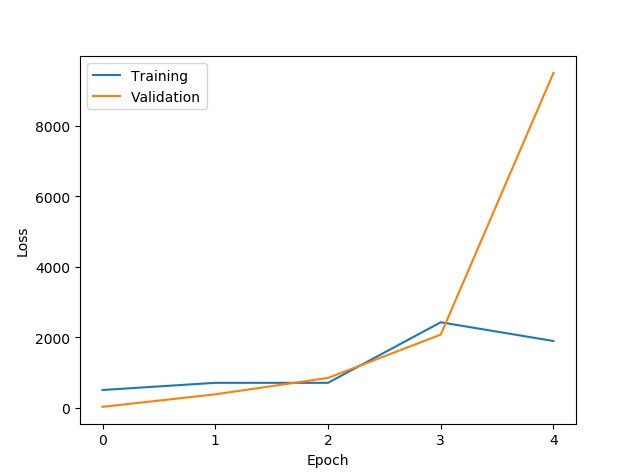
\includegraphics[width=9cm]{adam64-5LR0.5.jpg}}\\
Loss graph for Second setting by each epoch.   
    \end{figure}

The second setting uses Adam Optimizer which is a more powerful optimizer than SGD. As a result, the final accuracy is much better than using SGD. However, 
I find that the validation curve is not very stable among several trials, because large learning rate causes overfitting problem and can only simulate training set
instead of generally classifying all possible data.

\newpage
\noindent
\textbf{Third setting}:\\
Preprocessor: SnowballStemmer set language to english, WordPunctTokenizer\\
CountVectorizer: set stopwords to english, max features to 5000\\
FastText: hidden neurons set to 64\\
Optimizer: Adam set lr to 0.001\\
Epoch set to 5\\
\\
\noindent
Training accuracy: 0.868869960308075\\
Validation accuracy: 0.8369536399841309\\
Testing accuracy: 0.8298999667167664\\
\begin{figure}[htp]
    \centering
    \center{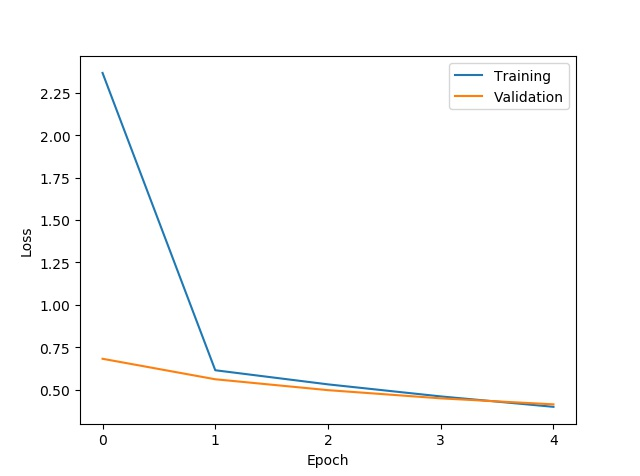
\includegraphics[width=9cm]{adam64-5LR0.001.jpg}}\\
Loss graph for Third setting by each epoch.   
    \end{figure}

The third setting uses Adam Optimizer and a fairly small learning rate to 0.001. In this setting, the validation process is stable during training, which means that smaller learning rate can prevent this model from overfitting problem and therefore it has better accuracy. However the model can't learn enough from training data due to small learning rate.


\noindent
\textbf{Forth setting}:\\
Preprocessor: SnowballStemmer set language to english, WordPunctTokenizer\\
CountVectorizer: set stopwords to english, max features to 5000\\
FastText: hidden neurons set to 64\\
Optimizer: Adam set lr to 0.01\\
Epoch set to 5\\
\\
\noindent
Training accuracy: 0.8751111030578613\\
Validation accuracy: 0.8643390536308289\\
Testing accuracy: 0.8671000003814697\\
\begin{figure}[htp]
    \centering
    \center{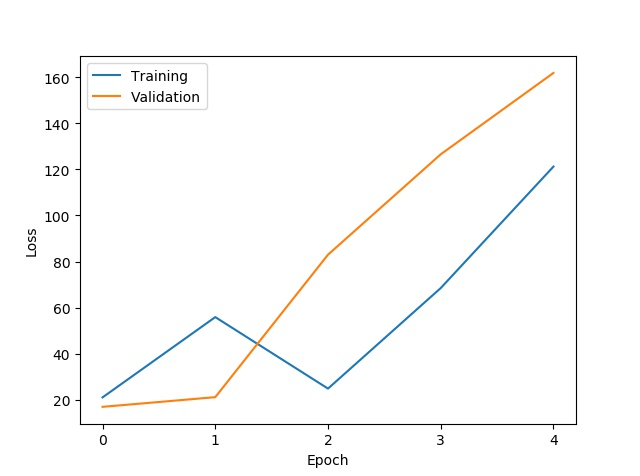
\includegraphics[width=9cm]{adam64-5LR0.1.jpeg}}\\
Loss graph for Forth setting by each epoch.   
    \end{figure}
The Forth setting I use is Adam Optimizer with learning rate to 0.1. Here the model still has a bit overfitting but we got a trade-off between overfitting and 
higher accuracy. Although small learning rate can prevent overfitting, the model may not have good accuracy because the model has not learned enough features with small learning rate and few epochs.

\noindent
\textbf{Fifth setting}:\\
Preprocessor: SnowballStemmer set language to english, WordPunctTokenizer\\
CountVectorizer: set stopwords to english, max features to 5000\\
FastText: hidden neurons set to 128\\
Optimizer: Adam set lr to 0.001\\
Epoch set to 10\\
\\
\noindent
training accuracy: 0.9328136444091797\\
validation accuracy: 0.8872379660606384\\
testing accuracy: 0.8869499564170837\\
\begin{figure}[htp]
    \centering
    \center{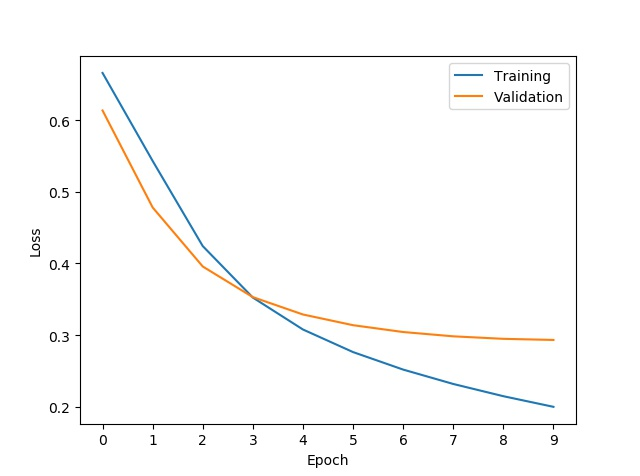
\includegraphics[width=9cm]{adam128-10LR0.001.jpg}}\\
Loss graph for Fifth setting by each epoch.   
    \end{figure}
    \\
The final setting I use is to handle both overfitting and accuracy. Firstly, to learn more features from training data, I set more epochs and smaller learning rate to fit the data with more steps and make full use of sparse data in training set. Also, more hidden neurons can make the model more expressive. Finally, the validation accuracy as well as testing accuracy reach a good balance point. The main advantage of the fifth setting over the forth is that model has more generalization ability from the training data and also prevents overfitting problem.


\section*{Question 4 Comparison of models}
LogisticRegression model performs better. LogisticRegression is used for classify 
whether candidate belongs to a certain class, movie review problem is a binary 
classify problem and LogisticRegression is suitable for this problem. What's more, movie review usually contains emotional words that  decides whether the review is positive or negative.


\section*{Question 5 Implement Word2Vec}
Code in Pycharm

\section*{Question 6 Compare pre-trained embeddings}
Classifier without pre-train performs better.

\section*{Question 7 Further Modification}


\end{document}